\section{Deniability}
Anyone with access to Flickr.com can view and download the original images stored by FFS, both registered users on Flickr, and anonymous visitors. An example of how the profile might look is shown in Figure~\ref{fig:flickr_profile}. The images found on the account present little information about the filesystem. For users unaware of FFS who view the Flickr profile, they see different sizes of images with seemingly randomly generated pixel colors. However, for adversaries who know about the details of FFS, more information can be retrieved. For instance, they could assume that the most recently uploaded image to Flickr is representing the inode table. However, as we assume the adversary does not have access to the decryption key, they cannot read the data of the image and thus cannot verify that this is indeed the inode table. The exact number of files and directories in FFS cannot be known precisely without access to the content of the inode table. Even if the Flickr account has, for instance, 15 images stored, and we know that one represents the inode table and one represents the root directory, it is not possible to conclude if other images stores file data or directory data. The remaining 13 images in the example represent:
\begin{itemize}
	\item one single file, or
	\item one single directory, or
	\item 13 different files, or
	\item 13 different directories, or
	\item 1 directory and 12 different files, or
	\item 13 copies of the same file, et cetera.
\end{itemize}
It is also not possible to know if an image stored on Flickr has been uploaded by FFS or by the user manually to further diffuse the amount of data stored on the service. For instance, by encrypting random data using FFS's encoder and uploading the images to Flickr, but without saving the posts in the inode table or in a directories of FFS, the images will look indistinguishable from the other images on Flickr. Only with access to the decrypted inode table can one know if the image is stored in FFS or not. One drawback of storing images on Flickr that are not stored in FFS is that it decreases the storage capacity of FFS.

\begin{figure}[!ht]
	\begin{center}
	  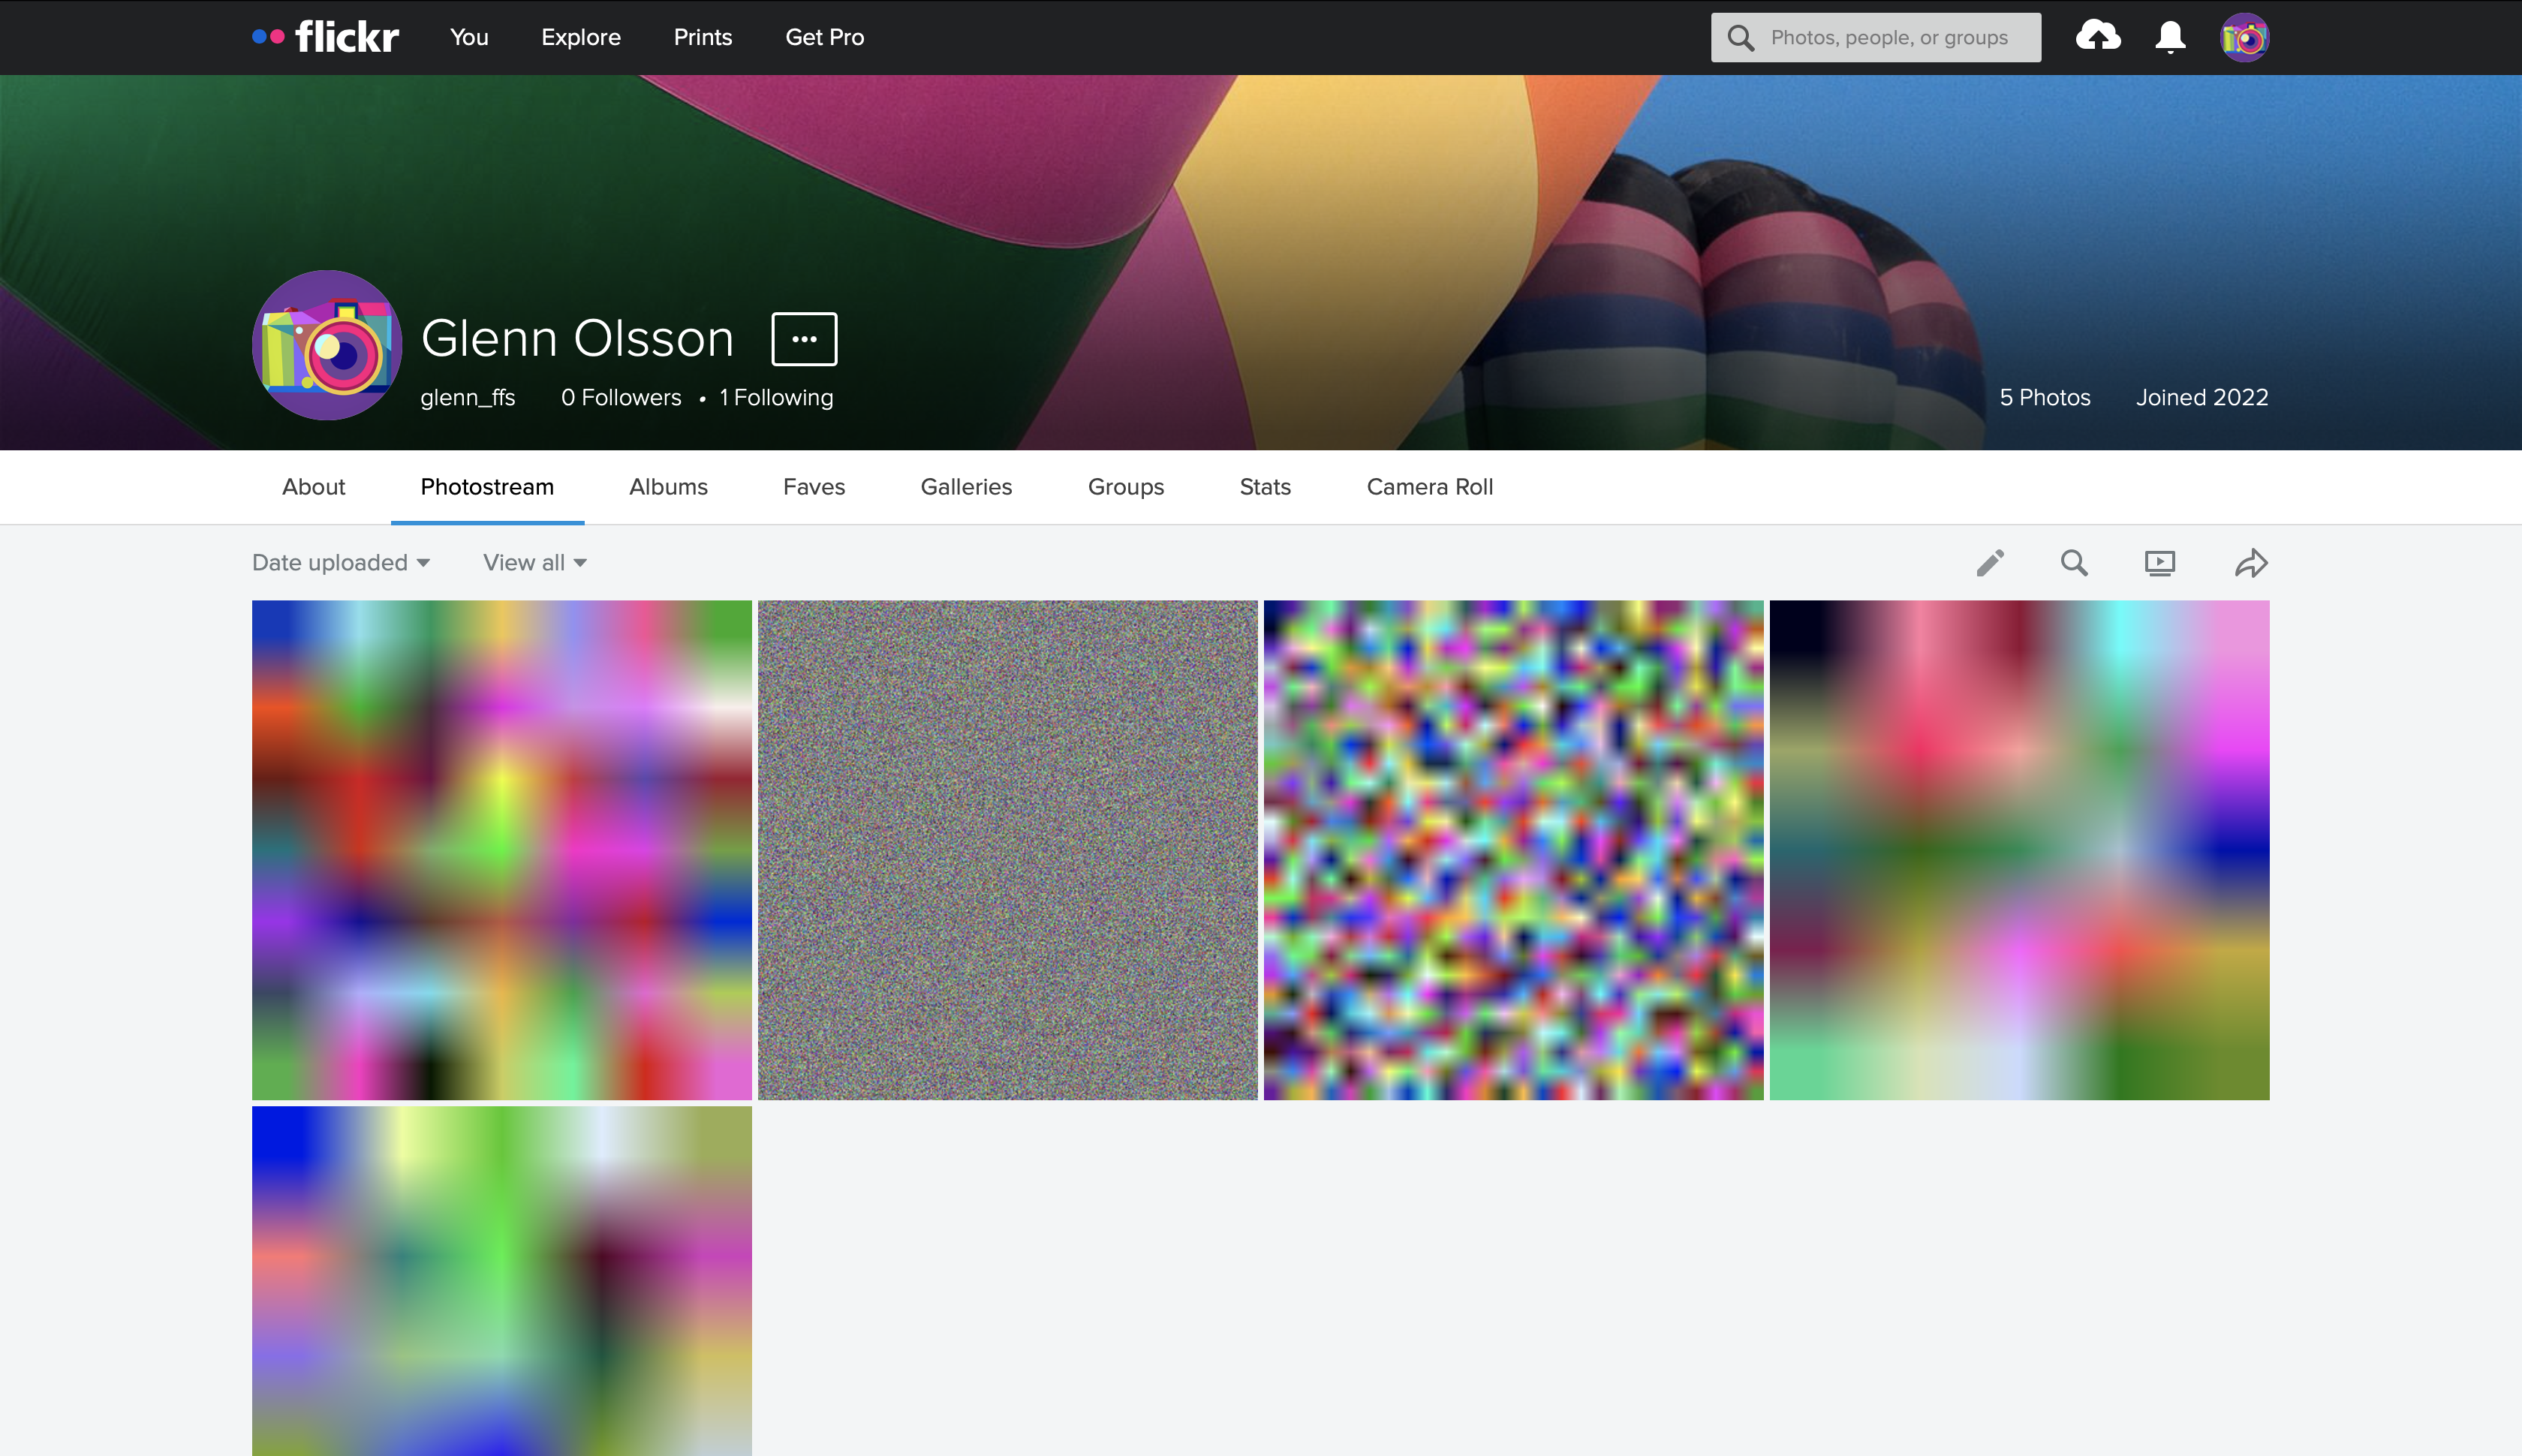
\includegraphics[width=0.8\textwidth]{figures/flickr_profile.png}
	\end{center}
	\caption[Screenshot of the Flickr profile used for FFS]{Screenshot of the Flickr profile used for FFS. At the moment of the screenshot, the filesystem is storing a previous version of this thesis in a directory inside the root directory. The images seen are the inode table, the thesis data, the root directory data, the subdirectory (containing the thesis) data, and a temporary file containing extra attributes of thesis document created by MacOS while FFS was mounted (this file is sometimes referred to as a \textit{turd}\,\cite{geekosaurAnswerWhyAre2011}).}
	\label{fig:flickr_profile}
\end{figure}

The size of data stored in an image is not completely hidden. While the exact number of bytes of unencrypted data that the image stores is not possible to know without the decryption key, it is possible to get an estimate. If you know the binary structure of the image (as presented in Appendix~\ref{app:binary_rep}), you can find out how many bytes the encrypted cipher is, the value of the IV data, the value of the salt used for the encryption key derivation, and the value of the authentication tag. By knowing the length of the cipher, the length of the unencrypted data can be placed in a range. The length of the cipher $L_c$ in bytes is divisible by 16 (as AES is a 16-byte block cipher), and the length of the plan text must be less than $L_c$ due to the requirement of at least one bit of padding\,\cite{z.z.coderAnswerSizeData2010}. The smallest possible size for the length of the plain text is $L_c - 16$. Therefore, the length of the plain text $L_p$ is:
$$
	L_c - 16 \leq L_p < L_c
$$
By examining all the images stored on Flickr and their maximum possible value of $L_p$, it is possible to know the largest possible amount of data which is stored by FFS on Flickr at a certain time. However, it is \textbf{not} possible to know if all this data is actually stored on FFS through entries in the inode table. It is also \textbf{not} possible to know if the plain text represents a file or directory without the decrypted data of the inode table.

If a user supplies a different password when mounting FFS than used previously, the images stored on Flickr cannot be decrypted. When FFS tries to read the image it believes represents the inode table (the most recently uploaded image) and it fails, it will simply create a new inode table representing an empty filesystem, and upload the image representing this inode table, essentially replacing the potentially previous inode table (if it existed). As it is not possible to know if the images already uploaded to Flickr represents an inode table without the correct decryption key, it is impossible to determine if the image that could have represented the inode table was indeed an inode table encrypted with another password, or if it was some arbitrary data. In a potential rubber-hose situation\footnote{When a adversary might torture the user, with for instance a rubber hose. See Section~\ref{sec:rubber_hose}}, the user of the filesystem could easily claim that they uploaded FFS images with arbitrary data, using randomly generated keys which they do not remember, and that the filesystem is empty. There is no way to prove the existence of any meaningful data on Flickr without the decryption key. As the FFS encoder also uses random salting for the encryption key, it is not even possible to prove that the images are encrypted with the same password as the encryption keys will differ for all images, even when the same password is used. 

As mentioned, we do however assume that an adversary has access to the structure of FFS images as well. To counter this, the user who wants to hide its data could, after creating a filesystem containing meaningful information, mount FFS again with another password. FFS would then create a new inode table and upload this table. In a rubber-hose situation, the user could give up the password to the most recently mounted FFS instance, which is empty. The adversary can verify that this password indeed decrypts the most recently uploaded image, and that the unencrypted image data represents an empty inode table. If the user proceeds to claim that they do not know the passwords of the other images, the adversary cannot prove that they contain meaningful data nor that they have been uploaded by the user. These images could, for instance, have been uploaded by another user of FFS.